% F089｜勾股整数数组的构造规律
% 保留上传模板中的 \Conclusion 与 01_function 引用层级；若项目实际模块目录不同，按真实目录调整前缀。
\Conclusion
\subsection{F089 勾股整数数组的构造规律}
% F089｜勾股整数数组的构造规律｜01_statement.tex
% 继承上传模板的 LaTeX 环境；当前条目的内容独立编写。
\clearpage
\begin{statementbox}
\textbf{\textcolor{CStatement}{有什么用：轻松造出整数直角三角形}}
\par\medskip
\begin{center}
% F089｜triangle 原创简明教学示意图
\begin{tikzpicture}[>=stealth,scale=.9]
\coordinate (A) at (0,0);\coordinate (B) at (4,0);\coordinate (C) at (0,3);
\fill[teal!12] (A)--(B)--(C)--cycle;\draw[very thick,teal] (A)--(B)--(C)--cycle;
\draw (.3,0)--(.3,.3)--(0,.3);
\node[below] at (2,0){$4$};\node[left] at (0,1.5){$3$};\node[right] at (2,1.6){$5$};
\node[anchor=west] at (5,2.1){$3^2+4^2=5^2$};
\node[anchor=west] at (5,1.3){\small 直角边的平方和};
\node[anchor=west] at (5,.8){\small 等于斜边平方};
\end{tikzpicture}

\end{center}
\medskip
已知 $3,4,5$ 满足 $3^2+4^2=5^2$，那么还能不能系统地制造 $5,12,13$、$8,15,17$？当然可以：只要取两个整数 $m>n\ge1$。
\end{statementbox}
\clearpage
\begin{statementbox}
\textbf{\textcolor{CStatement}{核心构造公式}}
\par\medskip
\begin{center}
% F089｜formula 原创简明教学示意图
\begin{tikzpicture}[>=stealth,scale=.9]
\node[draw,rounded corners,fill=teal!9] (a) at (0,0) {$m>n>0$};
\node[draw,rounded corners,fill=orange!10] (b) at (4.5,0) {$m^2-n^2,\ 2mn,\ m^2+n^2$};
\draw[->,thick] (a)--(b);
\node at (4.5,-1){\small 任取正整数 $m>n$，都会得到一组勾股数};
\end{tikzpicture}

\end{center}
\medskip
\[\boxed{(a,b,c)=(m^2-n^2,\ 2mn,\ m^2+n^2)},\qquad m>n\ge1.\]其中 $a,b$ 是直角边，$c$ 是斜边。取 $m=2,n=1$：得到 $(3,4,5)$；取 $m=3,n=2$：得到 $(5,12,13)$。
\end{statementbox}

% F089｜勾股整数数组的构造规律｜02_explanation.tex
% 继承上传模板的 LaTeX 环境；当前条目的内容独立编写。
\clearpage
\begin{explanationbox}
\textbf{\textcolor{CExplanation}{为什么一定能构成直角三角形}}
\par\medskip
\begin{center}
% F089｜triangle 原创简明教学示意图
\begin{tikzpicture}[>=stealth,scale=.9]
\coordinate (A) at (0,0);\coordinate (B) at (4,0);\coordinate (C) at (0,3);
\fill[teal!12] (A)--(B)--(C)--cycle;\draw[very thick,teal] (A)--(B)--(C)--cycle;
\draw (.3,0)--(.3,.3)--(0,.3);
\node[below] at (2,0){$4$};\node[left] at (0,1.5){$3$};\node[right] at (2,1.6){$5$};
\node[anchor=west] at (5,2.1){$3^2+4^2=5^2$};
\node[anchor=west] at (5,1.3){\small 直角边的平方和};
\node[anchor=west] at (5,.8){\small 等于斜边平方};
\end{tikzpicture}

\end{center}
\medskip
把斜边平方展开：$(m^2+n^2)^2=m^4+2m^2n^2+n^4$。两直角边平方之和是 $(m^2-n^2)^2+(2mn)^2=m^4+2m^2n^2+n^4$，正好相等。
\end{explanationbox}
\clearpage
\begin{explanationbox}
\textbf{\textcolor{CExplanation}{奇数平方拆成两个相邻数}}
\par\medskip
\begin{center}
% F089｜odd 原创简明教学示意图
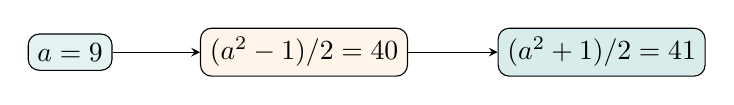
\begin{tikzpicture}[>=stealth,scale=.9]
\node[draw,fill=teal!10,rounded corners] (a) at (0,0){$a=9$};
\node[draw,fill=orange!8,rounded corners] (b) at (3.3,0){$(a^2-1)/2=40$};
\node[draw,fill=teal!15,rounded corners] (c) at (7.5,0){$(a^2+1)/2=41$};
\draw[->] (a)--(b);\draw[->] (b)--(c);
\end{tikzpicture}

\end{center}
\medskip
若直角边 $a$ 为大于1的奇数，则 $a^2$ 为奇数。令另两边为 $b$ 和 $b+1$，由 $a^2+(b)^2=(b+1)^2$，可得 $a^2=2b+1$，所以 $b=(a^2-1)/2$。例如 $a=9$ 得 $(9,40,41)$。
\end{explanationbox}
\clearpage
\begin{explanationbox}
\textbf{\textcolor{CExplanation}{偶数半数平方加减1}}
\par\medskip
\begin{center}
% F089｜even 原创简明教学示意图
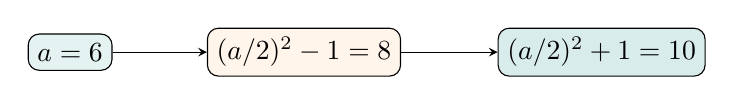
\begin{tikzpicture}[>=stealth,scale=.9]
\node[draw,fill=teal!10,rounded corners] (a) at (0,0){$a=6$};
\node[draw,fill=orange!8,rounded corners] (b) at (3.3,0){$(a/2)^2-1=8$};
\node[draw,fill=teal!15,rounded corners] (c) at (7.5,0){$(a/2)^2+1=10$};
\draw[->] (a)--(b);\draw[->] (b)--(c);
\end{tikzpicture}

\end{center}
\medskip
若 $a=2n$ 且 $n\ge2$，则 $(n^2+1)^2-(n^2-1)^2=4n^2=a^2$。例如 $a=8$，$n=4$，得到 $(8,15,17)$。
\end{explanationbox}

% F089｜勾股整数数组的构造规律｜03_proof.tex
% 继承上传模板的 LaTeX 环境；当前条目的内容独立编写。
\clearpage
\begin{proofbox}
\textbf{\textcolor{CProof}{证明一（最快）：直接平方展开}}
\par\medskip
\begin{center}
% F089｜formula 原创简明教学示意图
\begin{tikzpicture}[>=stealth,scale=.9]
\node[draw,rounded corners,fill=teal!9] (a) at (0,0) {$m>n>0$};
\node[draw,rounded corners,fill=orange!10] (b) at (4.5,0) {$m^2-n^2,\ 2mn,\ m^2+n^2$};
\draw[->,thick] (a)--(b);
\node at (4.5,-1){\small 任取正整数 $m>n$，都会得到一组勾股数};
\end{tikzpicture}

\end{center}
\medskip
\[(m^2-n^2)^2+(2mn)^2\]$=m^4-2m^2n^2+n^4+4m^2n^2$ $=m^4+2m^2n^2+n^4=(m^2+n^2)^2$。因此总是勾股整数数组。
\end{proofbox}
\clearpage
\begin{proofbox}
\textbf{\textcolor{CProof}{证明二（最低门槛）：奇数公式}}
\par\medskip
\begin{center}
% F089｜odd 原创简明教学示意图
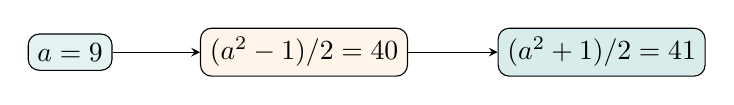
\begin{tikzpicture}[>=stealth,scale=.9]
\node[draw,fill=teal!10,rounded corners] (a) at (0,0){$a=9$};
\node[draw,fill=orange!8,rounded corners] (b) at (3.3,0){$(a^2-1)/2=40$};
\node[draw,fill=teal!15,rounded corners] (c) at (7.5,0){$(a^2+1)/2=41$};
\draw[->] (a)--(b);\draw[->] (b)--(c);
\end{tikzpicture}

\end{center}
\medskip
令奇数 $a\ge3$，取 $b=(a^2-1)/2,c=(a^2+1)/2$。两数相差1，因此 $c^2-b^2=(c-b)(c+b)=1\cdot a^2=a^2$，即 $a^2+b^2=c^2$。
\end{proofbox}
\clearpage
\begin{proofbox}
\textbf{\textcolor{CProof}{证明三（步骤最少）：偶数公式}}
\par\medskip
\begin{center}
% F089｜even 原创简明教学示意图
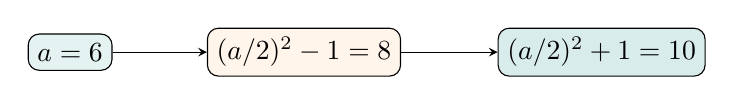
\begin{tikzpicture}[>=stealth,scale=.9]
\node[draw,fill=teal!10,rounded corners] (a) at (0,0){$a=6$};
\node[draw,fill=orange!8,rounded corners] (b) at (3.3,0){$(a/2)^2-1=8$};
\node[draw,fill=teal!15,rounded corners] (c) at (7.5,0){$(a/2)^2+1=10$};
\draw[->] (a)--(b);\draw[->] (b)--(c);
\end{tikzpicture}

\end{center}
\medskip
令 $a=2n$，其中 $n\ge2$；取 $b=n^2-1,c=n^2+1$，由平方差得 $c^2-b^2=(c-b)(c+b)=2\times2n^2=4n^2=a^2$。
\end{proofbox}

% F089｜勾股整数数组的构造规律｜04_examples.tex
% 继承上传模板的 LaTeX 环境；当前条目的内容独立编写。
\clearpage
\begin{examplebox}
\textbf{\textcolor{CExample}{例 1：构造5,12,13}}
\par\medskip
\begin{center}
% F089｜formula 原创简明教学示意图
\begin{tikzpicture}[>=stealth,scale=.9]
\node[draw,rounded corners,fill=teal!9] (a) at (0,0) {$m>n>0$};
\node[draw,rounded corners,fill=orange!10] (b) at (4.5,0) {$m^2-n^2,\ 2mn,\ m^2+n^2$};
\draw[->,thick] (a)--(b);
\node at (4.5,-1){\small 任取正整数 $m>n$，都会得到一组勾股数};
\end{tikzpicture}

\end{center}
\medskip
取 $m=3,n=2$：$m^2-n^2=9-4=5$，$2mn=12$，$m^2+n^2=13$。所以 $5^2+12^2=13^2$。
\end{examplebox}
\clearpage
\begin{examplebox}
\textbf{\textcolor{CExample}{例 2：给出奇数9，马上得三边}}
\par\medskip
\begin{center}
% F089｜odd 原创简明教学示意图
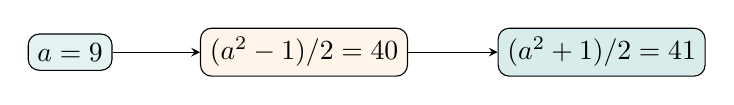
\begin{tikzpicture}[>=stealth,scale=.9]
\node[draw,fill=teal!10,rounded corners] (a) at (0,0){$a=9$};
\node[draw,fill=orange!8,rounded corners] (b) at (3.3,0){$(a^2-1)/2=40$};
\node[draw,fill=teal!15,rounded corners] (c) at (7.5,0){$(a^2+1)/2=41$};
\draw[->] (a)--(b);\draw[->] (b)--(c);
\end{tikzpicture}

\end{center}
\medskip
$a=9$，另外两边为 $(81-1)/2=40$ 和 $(81+1)/2=41$，得到 $\boxed{(9,40,41)}$。
\end{examplebox}
\clearpage
\begin{examplebox}
\textbf{\textcolor{CExample}{例 3：给出偶数10，马上得三边}}
\par\medskip
\begin{center}
% F089｜even 原创简明教学示意图
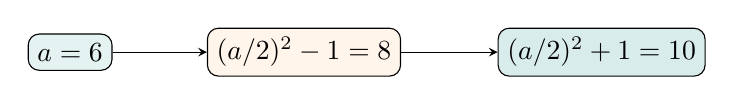
\begin{tikzpicture}[>=stealth,scale=.9]
\node[draw,fill=teal!10,rounded corners] (a) at (0,0){$a=6$};
\node[draw,fill=orange!8,rounded corners] (b) at (3.3,0){$(a/2)^2-1=8$};
\node[draw,fill=teal!15,rounded corners] (c) at (7.5,0){$(a/2)^2+1=10$};
\draw[->] (a)--(b);\draw[->] (b)--(c);
\end{tikzpicture}

\end{center}
\medskip
$a=10=2\times5$，另外两边 $25-1=24$、$25+1=26$，得到 $\boxed{(10,24,26)}$。
\end{examplebox}

% F089｜勾股整数数组的构造规律｜05_traps.tex
% 继承上传模板的 LaTeX 环境；当前条目的内容独立编写。
\clearpage
\begin{trapbox}
\textbf{\textcolor{CTrap}{易错一：把生成的一组当成全部}}
\par\medskip
\begin{center}
% F089｜odd 原创简明教学示意图
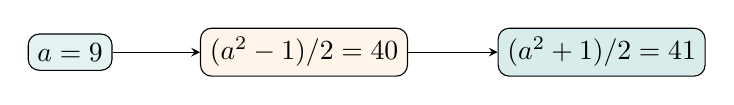
\begin{tikzpicture}[>=stealth,scale=.9]
\node[draw,fill=teal!10,rounded corners] (a) at (0,0){$a=9$};
\node[draw,fill=orange!8,rounded corners] (b) at (3.3,0){$(a^2-1)/2=40$};
\node[draw,fill=teal!15,rounded corners] (c) at (7.5,0){$(a^2+1)/2=41$};
\draw[->] (a)--(b);\draw[->] (b)--(c);
\end{tikzpicture}

\end{center}
\medskip
已知直角边为 $9$，奇数快捷式给出 $(9,40,41)$，但 $(9,12,15)$ 也成立。若题目问\textbf{所有组合}，必须用 F090 的因数配对法。
\end{trapbox}
\clearpage
\begin{trapbox}
\textbf{\textcolor{CTrap}{易错二：m和n随便取}}
\par\medskip
\begin{center}
% F089｜formula 原创简明教学示意图
\begin{tikzpicture}[>=stealth,scale=.9]
\node[draw,rounded corners,fill=teal!9] (a) at (0,0) {$m>n>0$};
\node[draw,rounded corners,fill=orange!10] (b) at (4.5,0) {$m^2-n^2,\ 2mn,\ m^2+n^2$};
\draw[->,thick] (a)--(b);
\node at (4.5,-1){\small 任取正整数 $m>n$，都会得到一组勾股数};
\end{tikzpicture}

\end{center}
\medskip
必须是正整数且 $m>n$；若 $m=n$，则 $m^2-n^2=0$，不再是正整数直角三角形。
\end{trapbox}
\clearpage
\begin{trapbox}
\textbf{\textcolor{CTrap}{易错三：所有构造结果都互质？}}
\par\medskip
\begin{center}
% F089｜triangle 原创简明教学示意图
\begin{tikzpicture}[>=stealth,scale=.9]
\coordinate (A) at (0,0);\coordinate (B) at (4,0);\coordinate (C) at (0,3);
\fill[teal!12] (A)--(B)--(C)--cycle;\draw[very thick,teal] (A)--(B)--(C)--cycle;
\draw (.3,0)--(.3,.3)--(0,.3);
\node[below] at (2,0){$4$};\node[left] at (0,1.5){$3$};\node[right] at (2,1.6){$5$};
\node[anchor=west] at (5,2.1){$3^2+4^2=5^2$};
\node[anchor=west] at (5,1.3){\small 直角边的平方和};
\node[anchor=west] at (5,.8){\small 等于斜边平方};
\end{tikzpicture}

\end{center}
\medskip
不一定。例如 $m=3,n=1$ 得到 $(8,6,10)$，三数可同时除以2。构造公式保证勾股关系，\textbf{不保证三边没有公因数}。
\end{trapbox}

% F089｜勾股整数数组的构造规律｜06_summary.tex
% 继承上传模板的 LaTeX 环境；当前条目的内容独立编写。
\clearpage
\begin{summarybox}
\textbf{\textcolor{CSummary}{快记、快懂、快用}}
\par\medskip
\begin{center}
% F089｜formula 原创简明教学示意图
\begin{tikzpicture}[>=stealth,scale=.9]
\node[draw,rounded corners,fill=teal!9] (a) at (0,0) {$m>n>0$};
\node[draw,rounded corners,fill=orange!10] (b) at (4.5,0) {$m^2-n^2,\ 2mn,\ m^2+n^2$};
\draw[->,thick] (a)--(b);
\node at (4.5,-1){\small 任取正整数 $m>n$，都会得到一组勾股数};
\end{tikzpicture}

\end{center}
\medskip
\textbf{快记：}$m^2-n^2,2mn,m^2+n^2$。\par\textbf{快懂：}展开后两边平方和恒等于斜边平方。\par\textbf{快用：}要“造一组”用 F089；要“找全组”用 F090。
\end{summarybox}
\clearpage
\begin{summarybox}
\textbf{\textcolor{CSummary}{奇偶直角边一眼记}}
\par\medskip
\begin{center}
% F089｜odd 原创简明教学示意图
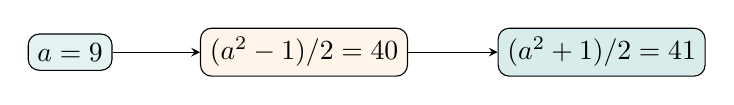
\begin{tikzpicture}[>=stealth,scale=.9]
\node[draw,fill=teal!10,rounded corners] (a) at (0,0){$a=9$};
\node[draw,fill=orange!8,rounded corners] (b) at (3.3,0){$(a^2-1)/2=40$};
\node[draw,fill=teal!15,rounded corners] (c) at (7.5,0){$(a^2+1)/2=41$};
\draw[->] (a)--(b);\draw[->] (b)--(c);
\end{tikzpicture}

\end{center}
\medskip
\textbf{奇数：}先平方，再一减一加后都除2。\par\textbf{偶数：}先取一半，再平方，最后减1和加1。\par\textbf{检查：}直角边都大于0，结果确为整数。
\end{summarybox}

